%!TEX root = ../Demo.tex
\chapter{引言}
\section{研究目的和意义}
不论在任何国家或地区,视频监控深入每个人的生活,视频监控的作用和能力也越来越强大。
从前,视频监控的唯一作用就是用来监视,记录过去一段时间发生的事情。
但是如今视频监控的作用不仅仅局限于此,还提供了例如交通违法抓拍、人脸识别辨别逃犯、
停车场车牌识别等等,它在安防领域发挥着不容小觑的作用,
对于保障人们日常生产和生活的安全具有重要意义,是大型企业诸如集团化公司、邮电、银行等信息交流广泛的企业生产和管理的必备系统。

近些年来,人们生活水平的提高,监控摄像头不仅仅只出现在公共场所,
老百姓的私人空间也会出现监控摄像头的身影。对于公共场所的监控,
产生的视频数据以及副产物会有相关部门管理,而且这类监控设备多用电子线缆传送数据,
会受到时间和地域的限制;老百姓家中的监控摄像头管理就相对分散,需要有个一平台提供在线观看、
视频回放等功能,因为不可能在每个用了这类摄像头的老百姓家中塞一个视频监控的查看终端。
因此催生了网络摄像头和网络视频监控系统。网络视频监控系统不仅可以用于公共摄像头,
也可以为私人的摄像头提供服务。

以网络为基础的视频监控突破了对时间、地域的限制,只要有网络存在的地方就可以建立网络监控系统,
省去了传统的布线和线路维护费用,降低了监控成本;用户在授权的情况下,
就可以不受地域时间限制随时按需监控,实现即插、即用、即看。


%视频监控技术的发展,给人们的生活和生产带来了极大的便利和充分的安全保障。
%视频监控系统是安防领域中的研究热点,随着近年来各类智能设备数量的爆发性增长,视频监控系统正朝着数字化、智能化、网络化、人性化的方向发展。
%随着人们生活水平的提高,人们更多的把目光投向了如何更好的保护自己和家人的人身安全以及经济财产,因此以前只出现在公共场所的监控摄像头,如今在人们的家中就能看到它们的身影,希望通过它们可以随时随地的对人或物进行安放监控。

%视频实时监控系统是一个可以实时对远程监控摄像头采集的画面进行实时监测的平台。
%Web端的视频实时监控系统可以依托手机、电脑等支持网页访问的设备进行查看,可以做到只要有网络,就可以随时随地查看监控视频。
%传统的视频监控系统需要在一个局域网内,在一台终端机器上才能实现监控视频的查看。
%本文提出了一种基于Spring Boot的视频实时监控系统的设计思路以及实现方法。


\section{视频监控发展现状}

\subsection{研究现状}
视频监控的兼容性。视频监控的普及非常迅速,现在几乎家家户户都会有一个或几个监控摄像头,
这些摄像头可能是同一家公司的产品,也可能不是用一家公司的产品。问题其实就出在这里,
每一家公司都有自己的协议,公司A需要在它自家的平台上才能看到队友监控视频,公司B也是如此。
这是因为现在的网络视频监控还没有一个统一个标准,做不到兼容所有的厂家,
或者说是每个厂家的生产都没有一个统一标准。

视频监控的智能化。现在市面上已经存在很多智能的监控摄像头它们具有目标追踪、人物检测等功能。
这大大减少了人力成本,比如以前需要手动去调整摄像头的朝向来跟踪一个目标,
但是现在这个是有机器自动操作。因此要想转变原本的人力监控,就需要进一步改进当前的视频监控和分析技术,
通过视觉技术来分析视频的背景和目标,从而实现目标智能化监控。

\subsection{发展趋势}
视频监控支持移动场景。传统的视频监控摄像头大多是固定不动的,可以认为是固定在某一个静止的物体上,
例如房屋的墙上、路灯杆上等等。在这种场景下,可以通过网络布线的方式解决监控中心与被监控点的通信。
但是一旦遇上部署在移动物体上的监控摄像头,例如公交车、高铁等,传统的网络布线方式解决通信问题
显然不可取,还有一种场景就是遇上了复杂地形,高山深谷、河流沙漠等等,同样有限网络也是束手无策。
这个时候支持移动网络的监控摄像头就显得尤为重要,3G、4G、5G等移动网络技术的出现,使得视频监控
支持移动场景变得更加简单。

视频监控支持 IPv6 协议。众所周知,IPv4 的地址已经耗尽,想在公网上继续增加新的 IPv4 地址的网
络监控摄像头有点困难,如果是在局域网中搭建的监控摄像头系统,那么就不会收到这个限制,但是局域网
中的监控摄像头只能在局域网中查看(排除将监控视频上传的公网的情况)。
视频监控支持家庭数字化。数字家庭网络可以由一个的统一的公共网管控制家中的所有智能家居,在视频监控
普及的过程中,不可避免的要和智能家居这个概念联系起来。最终的结果就是视频监控也能支持家庭数字化的
场景,能使用一个统一网关进行操作(观看实时录像、视频回放、抓拍等功能)。

\section{本文主要工作}
为了满足视频监控系统数字化、智能化、网络化、人性化发展的需求,
本文基于Spring Boot设计并实现了一个视频实时监控系统。本系统将传统的视频监控系统与网页结合,
拥有链接安防摄像头、查看实时视频、视频保存和查看功能。

系统主要分为服务器端和网页客户端。
服务器端主要使用Spring Boot 编写实现,采用 HTTP 协议与网页客户端交互,接口依照 RESTful 风格编写,
并使用 Java-CV依赖对摄像头视频数据进行采集保存。网页客户端主要使用Vue.js框架编写,主要实现了用户登录、实时监控查看、监控回放查看、增减设备、个人中心、权限管理等功能。
总的来说,本文的主要工作可以概括为一下几点:
\begin{enumerate}
    \item 链接安防摄像头,实时查看视频监控。通过安防摄像头厂商提供的 SDK,代码中引入并调用即可,可以对安防摄像头的视频数据进行读取。
    此外也可以直接使用网络摄像头自带的RTMP或者HTTP-FLV协议格式的视频流地址,实现对摄像头视频的查看和录制。
    \item 视频按时间顺序保存并支持检索。对从安防摄像头上获取的视频数据进行编码,
    保存MP4格式的视频文件到本地磁盘或者分布式存储系统中,以“安防摄像头唯一标识 + 视频时间”作为视频文件的文件名,
    以达到按时间存储的目的,同时在借助数据库保存视频文件的相关信息,支持根据视频文件的开始时间和结束时间为搜索条件进行检索。
    \item 用户登陆和权限管理。不同的用户对监控设备有不一样的可见权限,同时不同的用户对系统的菜单也有不同的可见权限。本文基于RBAC设计了一个权限系统。
    \item 前端页面开发和后端服务开发。前端页面采用 Vue.js框架 进行编写,采用 Element-UI 开源前端组件。后端采用  SpringBoot 框架实现服务,
    % 若后续技术分析中发现服务体量大,会采用 Consul 作为服务发现,用微服务的形式提供。
    采用前后端分离的方式实现,定义RESTful接口交互,实现解耦。
\end{enumerate}


\section{本文结构}
第一章介绍了本课题的研究目的和意义,简述了当前视频监控技术和视频监控系统的研究现状和发展趋势,最后对课题的主要工作进行了概括。

第二章介绍了系统设计过程中涉及到的关键技术。首先对流媒体传输技术进行了详细介绍,紧接着对开发框架Spring Boot、MapStruct和数据存储技术Redis进行了简要叙述。
最后介绍了RABC权限系统的概念以及设计思路。

第三章介绍了系统的总体设计思路。

第四章介绍了系统的具体开发实现细节。

\chapter{关键技术研究}
\section{流媒体传输技术}
实时的视频监控系统需要基于流媒体传输技术来实现,需要摄像头本身或者后置的图像处理服务器支持流媒体传输,常见的三种流媒体传输技术有:RTMP、HTTP-FLV和HLS。

\subsection{流媒体以及流式传输}
流媒体是指将一连串的媒体数据(包含音频、视频数据)压缩后,采用流式传输的方式发送数据,
在网上即时传输影音以供观赏的一种技术与过程,此技术使得数据包得以像流水一样发送;
如果不使用此技术,就必须在使用前下载整个媒体文件。
流媒体在播放前不会下载整个文件,只将开始部分存入内存,同时也会在用户访问时对数据包进行缓存,
让媒体数据正确地输出,流媒体数据流随时传送随时播放。

流式传输是指客户端通过链接流媒体服务器实时传输音频、视频数据,实现“边下载边播放”。
流式传输是实现流媒体的关键技术。
流式传输时,音频、视频等时基媒体由音视频服务器向用户计算机的连续、实时传送,
用户不必等到整个文件全部下载完毕,而只需经过几秒或十数秒的启动延时即可进行观看。
当音频、视频等时基媒体在客户机上播放时,文件的剩余部分将在后台从服务器内继续下载。
流式不仅使启动延时成十倍、百倍地缩短,而且不需要太大的缓存容量。
流式传输避免了用户必须等待整个文件全部从网络上下载才能观看的缺点。

\begin{figure}[ht]
    \centering
    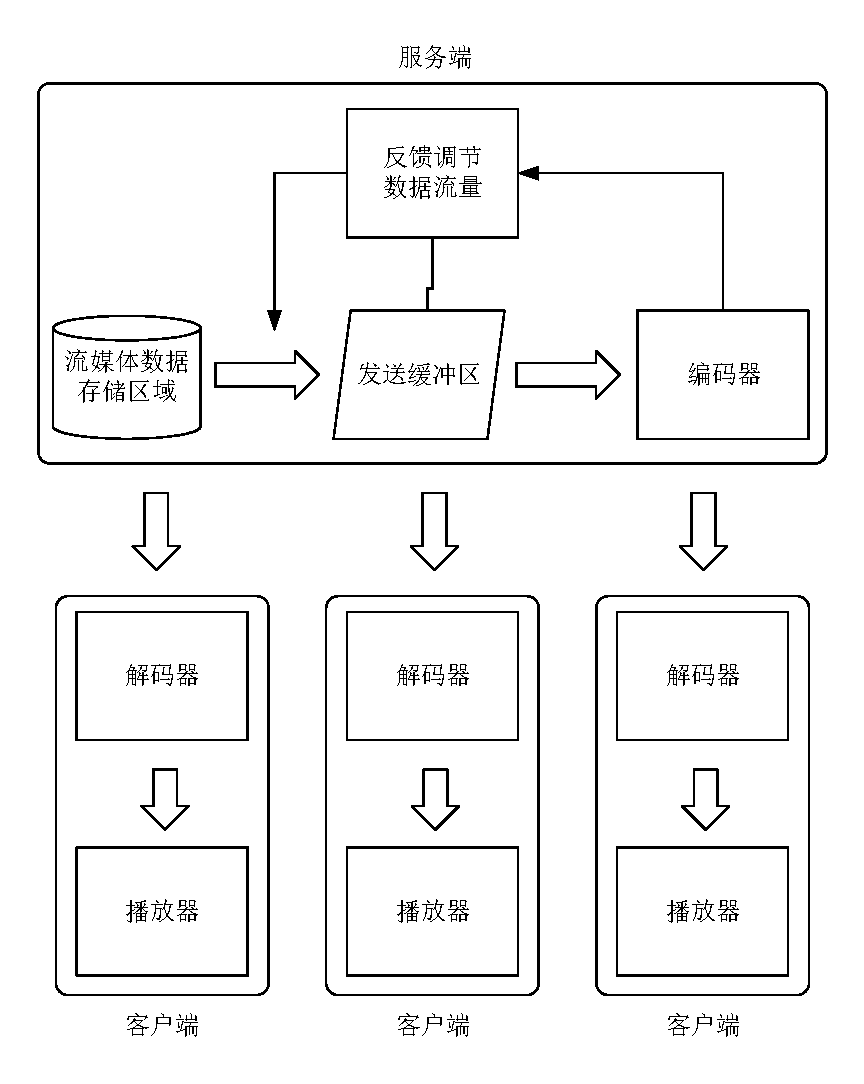
\includegraphics[scale=1]{./Figure/IMG_server.pdf}
    \caption{流式传输示意图}
    \label{Fig:server}
\end{figure}

图\ref{Fig:server} 展示了流式传输的工作过程。
流媒体数据存储区存放着视频、音频等多媒体数据,这些数据经过发送缓冲区,被编码器编码后发送给客户端。
发送缓冲区和编码器对发送的数据流量进行负反馈调节,防止因为网络拥塞造成卡顿或者数据丢失。
服务端和客户端之间通过流媒体传输协议交互。客户端收到服务端发送的数据之后,进行解码然后在播放器中播放。

% 在网络上传输音频、视频等多媒体信息,主要有下载和流式传输两种方案。
% 多媒体文件一般都较大,所以需要的存储容量也较大;
% 同时由于网络带宽的限制,通过下载实现的多媒体数据传输常常要花数分钟甚至数小时,
% 所以这种处理方法延迟也很大。

\subsection{基于RTMP的流媒体传输技术}
% 实时消息传输协议(即Real-Time Messaging Protocol,缩写RTMP) 最初是Macromedia公司为了满足在互联网上传输流媒体音视频而开发的一个私有协议。

% RTMP(Real Time Messaging Protocol) 是由 Adobe 公司基于 Flash Player 播放器对应的音视频 flv 封装格式提出的一种,基于TCP 的数据传输协议。本身具有稳定、兼容性强、高穿透的特点。常被应用于流媒体直播、点播等场景。

% RTMP(Real Time Messaging Protocol) 是由 Adobe 公司基于 Flash Player 播放器对应的音视频 flv 封装格式提出的一种,基于TCP 的数据传输协议。本身具有稳定、兼容性强、高穿透的特点。常被应用于流媒体直播、点播等场景。常用于推推流方(主播)的稳定传输需求

% RTMP,全称 Real Time Messaging Protocol,即实时消息传送协议,
% 最初是Macromedia公司为了满足在互联网上传输流媒体音视频而开发的一个私有协议。
实时消息传输协议(即Real-Time Messaging Protocol,缩写RTMP) 最初是Macromedia公司为了满足在互联网上传输流媒体音视频而开发的一个私有协议。
RTMP是工作在TCP之上的明文协议,默认使用端口1935。

RTMP 协议为了维持稳定连续传递,避免单次传输数据量问题,采用了传输层封包,数据流切片的实现形式。
被用来对当前带宽进行划分和复用的最小传输单位,被称为 Chunk 即消息块。

\begin{figure}[ht]
    \centering
    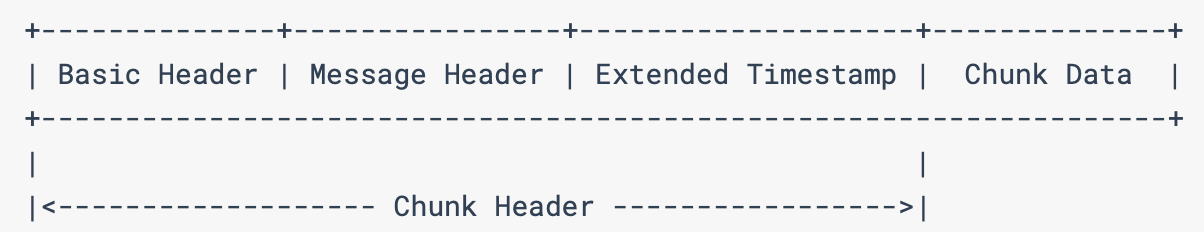
\includegraphics[scale=.4]{./Figure/IMG_chunk.png}
    \caption{Chunk 格式示意图}。
    \label{Fig:chunk}
\end{figure}

一个完整的数据块包含两个部分:Chunk Header 和 Chunk Data,
这两者组合在一起,构成了一个有效的消息类型,结构如图\ref{Fig:chunk}所示。
Chunk Header 由基础数据头(Basic Header)、消息数据头(Message Header)和
扩展时间戳(Extended Timestamp)构成。

通常情况下,一个有效的消息,如果数据量超出当前 Chunk Size 的话,则会被拆分成多个分块来分批传输。
默认情况下,Chunk Size 的值为 128字节。

\begin{figure}[ht]
    \centering
    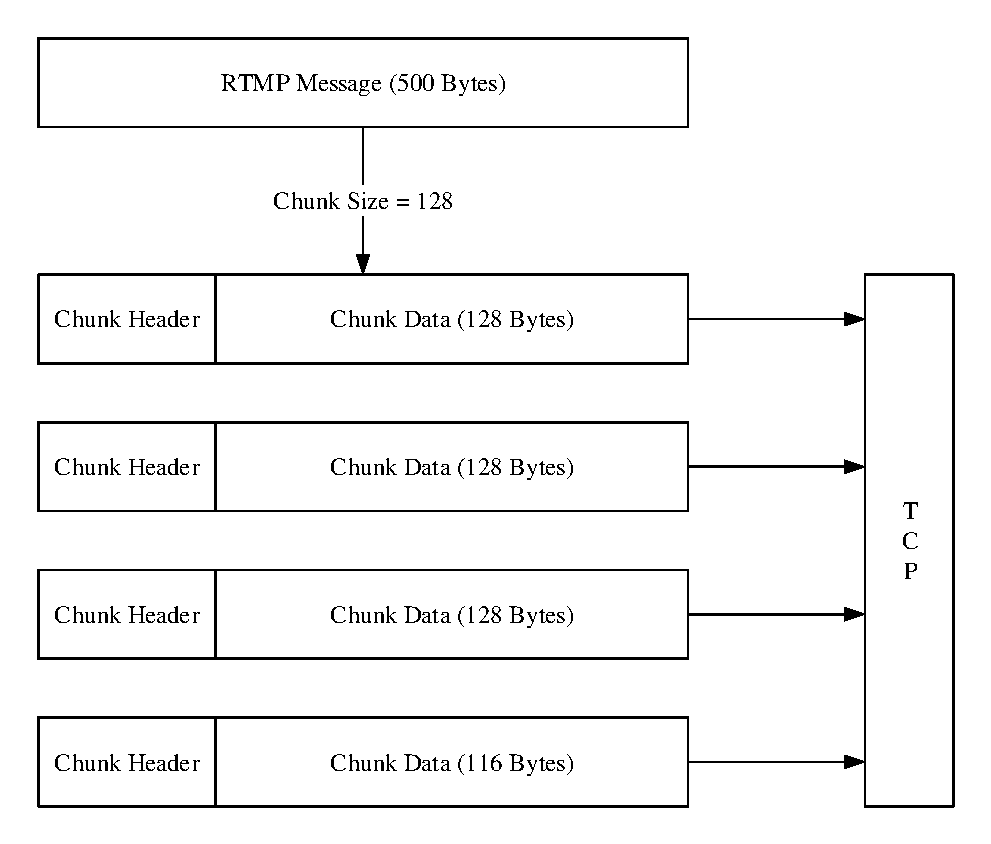
\includegraphics[scale=1]{./Figure/IMG_rtmp.pdf}
    \caption{消息拆分示意图}
    \label{Fig:rtmp}
\end{figure}
 
协议中的基本数据单元称为消息(Message),传输的过程中消息会被拆分为更小的消息块(Chunk)单元,
最后将分割后的消息块通过 TCP 协议传输,接收端再反解接收的消息块恢复成流媒体数据。
图 \ref{Fig:rtmp} 展示了一则当Chunk Size为128字节是的消息拆分发送过程。
一个大小为 500 字节的 RTMP消息,被拆分为4个大小分别为128字节、128字节、
128字节、116字节的消息块,最终通过TCP发送出去。

% 通过指定首个 Chunk 和后续 Chunk 类型,以及 Chunk Header 其他标志性数据,来使当前被切割的消息,能够在对端得到有效的还原和执行。我们以 MetaData 类型消息(Data AFM3 16)举例:

RTMP主要有以下几个优点:

\begin{enumerate}
    \item RTMP 是专门为流媒体开发的协议,对底层的优化比其它协议更加优秀。
    \item 基本上所有的编码器(摄像头之类)都支持 RTMP 输出,。
    \item RTMP适合长时间播放,并且具有较低的延时,一般延时在 1-3s 之间。
\end{enumerate}

RTMP并不是完美的,也有不足之处。
一方面是它是基于 TCP 传输,没有像HTTP那样的公共端口,被防火墙拦截的可能性也更大;
另一方面是Adobe并没有完全开源RTMP协议,这就导致很多设备无法需要使用第三方解码器才能播放。

\subsection{基于HTTP-FLV的流媒体传输技术}
FLV (Flash Video) 是 Adobe 公司推出的另一种视频格式,是一种在网络上传输的流媒体数据存储容器格式。其格式相对简单轻量,不需要很大的媒体头部信息。整个 FLV 由 The FLV Header, The FLV Body 以及其它 Tag 组成。因此加载速度极快。采用 FLV 格式封装的文件后缀为 .flv。

preview

而我们所说的 HTTP-FLV 即将流媒体数据封装成 FLV 格式,然后通过 HTTP 协议传输给客户端。

HTTP-FLV 依靠 MIME 的特性,根据协议中的 Content-Type 来选择相应的程序去处理相应的内容,使得流媒体可以通过 HTTP 传输。相较于 RTMP 协议,HTTP-FLV 能够好的穿透防火墙,它是基于 HTTP/80 传输,有效避免被防火墙拦截。除此之外,它可以通过 HTTP 302 跳转灵活调度/负载均衡,支持使用 HTTPS 加密传输,也能够兼容支持 Android,iOS 的移动端。

说了这么多优点,也来顺便说下 HTTP-FLV 的缺点,由于它的传输特性,会让流媒体资源缓存在本地客户端,在保密性方面不够好。因为网络流量较大,它也不适合做拉流协议。

\subsection{基于HLS的流媒体传输技术}


上述两个协议都是有Adobe公司推出的,而下面要讲的 HLS (HTTP Live Streaming) 则是苹果公司基于 HTTP 的流媒体传输协议。主要应用于 iOS 设备,包含(iPhone, iPad, iPod touch) 以及 Mac OSX 提供音视频直播服务和录制内容(点播)等服务。

相对于常见的流媒体协议,HLS 最大的不同在于它并不是一下请求完整的数据流。它会在服务器端将流媒体数据切割成连续的时长较短的 ts 小文件,并通过 M3U8 索引文件按序访问 ts 文件。客户端只要不停的按序播放从服务器获取到的文件,从而实现播放音视频。

相较 RTMP 而言,使用 HLS 在 HTML5 页面上实现播放非常简单:

直接:

preview

或者:

preview

HLS 的优势:

Apple 的全系列产品支持:由于 HLS 是苹果提出的,所以在 Apple 的全系列产品包括 iPhone、 iPad、safari 都不需要安装任何插件就可以原生支持播放 HLS, 现在 Android 也加入了对 HLS 的支持。

穿透防火墙。基于 HTTP/80 传输,有效避免防火墙拦截

性能高。通过 HTTP 传输, 支持网络分发,CDN 支持良好,且自带多码率自适应,Apple 在提出 HLS 时,就已经考虑了码流自适应的问题。

HLS 的劣势:

实时性差,延迟高。HLS 的延迟基本在 10s+ 以上

文件碎片。特性的双刃剑,ts 切片较小,会造成海量小文件,对存储和缓存都有一定的挑战



\subsection{RTMP、 HTTP-FLV、 HLS简单对比}
表\ref{Tab:pcompare} 对RTMP、 HTTP-FLV、 HLS这三种协议在底层传输协议、延迟、使用场景等方面进行了对比。

\begin{tabular}{ccccccc}
    \caption{RTMP、 HTTP-FLV、 HLS对比}
    \label{Tab:pcompare}\\
    \toprule
    协议&底层传输协议&视频封装格式&延迟&数据分段&HTML5&应用场景\\
    \midrule
    RTMP&TCP&flv tag&2秒&连续流&不支持&互动直播、点播、在线教育\\
    HTTP-FLV&HTTP&flv&2秒&连续流&支持&HTML5、互动直播、点播、在线教育\\
    HLS&HTTP&m3u8&10秒以上&切片&支持&HTML5、互动直播、点播、在线教育\\
    \bottomrule
\end{tabular}

RTMP 协议为流媒体而设计,在推流中用的比较多,同时大多 CDN 厂商支持RTMP 协议。

HTTP-FLV 使用类似 RTMP流式的 HTTP 长连接,需由特定流媒体服务器分发的,兼顾两者的优点。以及可以复用现有 HTTP 分发资源的流式协议。它的实时性和 RTMP 相等,与 RTMP 相比又省去了部分协议交互时间,首屏时间更短,可拓展的功能也更多。

HLS 作为苹果提出的直播协议,在 iOS 端占据了不可撼动的地位,Android 端也同时提供相应的支持。
\section{Spring Boot开发框架}
\subsection{Spring Boot开发框架简介}
Spring Boot是由Pivotal团队提供的全新框架,
其设计目的是用来简化新Spring应用的初始搭建以及开发过程。
该框架使用了特定的方式来进行配置,从而使开发人员不再需要定义样板化的配置。


Spring Boot不仅继承了Spring框架原有的优秀特性,而且还通过简化配置来进一步简化了Spring应用的整个搭建和开发过程。
在Spring Boot出现之前,使用Spring框架进行应用开发需要编写繁琐的配置文件,然而这些配置文件的内容大多都是类似的。

如图 \ref{Fig:spring} 所示,Spring框架约由20个模块组成,它们被分成
Core Container(核心容器)、
Data Access/Integration(数据访问集成)、
Web(网页)、
AOP(面向切面编程)、
Instrumentation(加载引入)、
Messaging(消息)
和Test(测试)七个大模块。

\begin{figure}[ht]
    \centering
    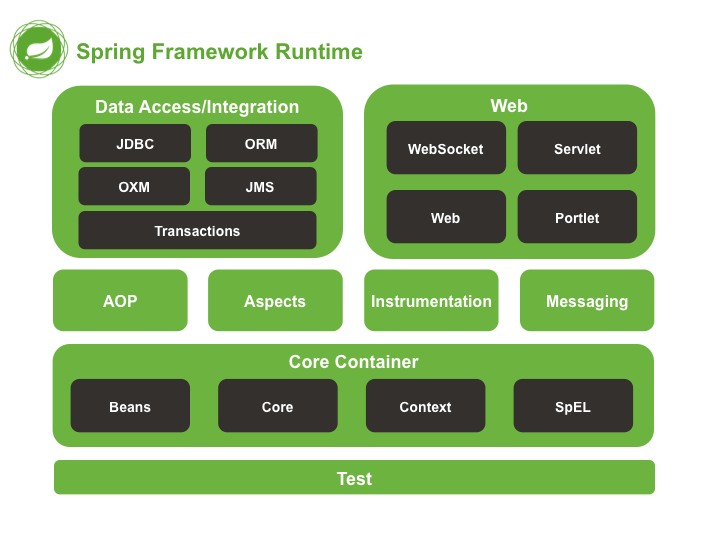
\includegraphics[scale=.4]{./Figure/IMG_spring.png}
    \caption{Spring框架模块结构}
    \label{Fig:spring}
\end{figure}

\begin{enumerate}
    %[label=(\arabic*)]
    \item Core Container 模块是 Spring 框架的基础,提供了控制反转(IoC)和依赖注入(DI)的能力。
    其内部的 BeanFactory 帮助开发者消除了手动创建单例的过程,将单例的创建和组装从业务代码中解耦。
    开发者可以通过ApplicationContext提供的接口访问容器内的创建的对象。
    容器同时还提供了表达式计算、第三方框架集成的能力。
    \item AOP and Instrumentation 模块提供了提供了面向切面编程以及第三方模块集成的能力。
    开发者可以通过面向切面编程可以通过方法拦截器或切点将非业务代码从业务代码中解耦。
    \item Messaging 模块提供了使用消息队列的统一接口。
    \item Data Access/Integration 模块由JDBC、ORM、OXM、JMS和Transaction构成。
    提供了屏蔽数据库供应商的数据库访问接口,并且支持事物。对象映射支持ORM、OXM等映射方式。
    同时还封装了面向消息队列的接口,支持对消息的生产和消费。
    \item Web 模块 提供了面向Web开发的基本功能的集成,例如基于其的Servlet加载、文件上传等功能。
    Web开发能力。可以借助该模块设计并实现一个基于MVC设计模式的Web应用程序。
    \item Test 模块提供了单元测试和集成测试的能力,使得普通的单元测试和集成测试也能使用Spring的容器。
\end{enumerate}

\subsection{控制反转和依赖注入特性简介}
Spring框架具有控制反转(IOC)特性,它通过对象元数据配置文件,借助Java反射机制提供的能力,
将程序生命周期周内的对象的创建和使用统一收口到Spring的容器中,由这个容器进行管理。

控制反转在大多数时候都是通过依赖注入来实现的。当对象A持有了类B的一个实例,就可以说对象A依赖对象B。
依赖注入要求对象与对象之间的依赖仅仅通过构造函数、工厂方法和属性写入方法来定义。
Spring容器就可以将通过这种方式声明的被依赖对象从容器中找到并且通过构造函数、工厂方法和属性写入方法来注入
到需要它的对象内。因为这个被依赖对象的创建过程是由容器完成的并在需要它的时候才进行注入,
而不是被需要它对象的创建的,所以这个过程就体现了控制反转和依赖注入。

\begin{figure}[ht]
    \centering   
    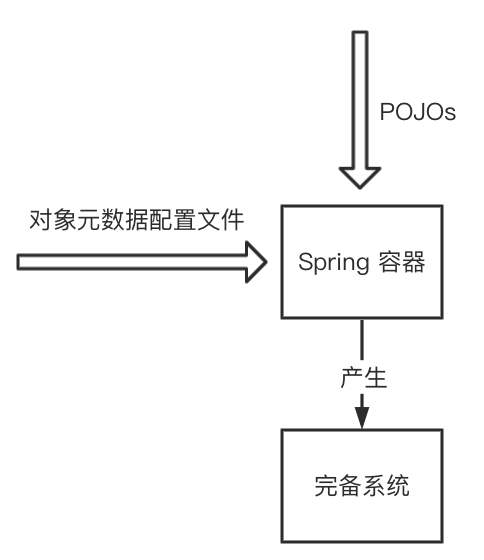
\includegraphics[scale=.3]{./Figure/IMG_container.png}
    \caption{IoC和DI工作过程}\label{Fig:erd}
\end{figure}

在Spring框架的定义中,控制反转又被称为依赖注入。


\subsection{面向切面编程简介}
Spring框架具有面向切面编程(AOP)框架,SpringAOP框架基于代理模式,同时运行时可配置;AOP框架主要针对模块之间的交叉关注点进行模块化。


\subsection{概述}

\subsection{控制反转特性}

\subsection{面向切面编程}


\section{对象拷贝技术MapStruct}

\section{内存数据库Redis}

\section{RBAC权限系统}


\chapter{系统总体设计}
本章将详细阐述系统的总体设计。
对毕业设计题目分析调研过后,可以将设计需求拆分为一下五点。


\section{实体关系设计}
本文的目标是设计并实现一个基于Spring Boot的视频实时监控系统。
一个完整的系统必然设计到用户,因此就需要用户实体。
由于是视频监控系统,那么有监控摄像头设备,因此需要设备实体。
此外还需要对监控摄像头产生的录像文件进行保存并支持检索,所以需要视频文件实体。

综上所示,本视频实时监控系统包括三个实体:用户、设备和视频文件。
本系统的实体关系图如下所示。

\begin{figure}[ht]
    \centering
    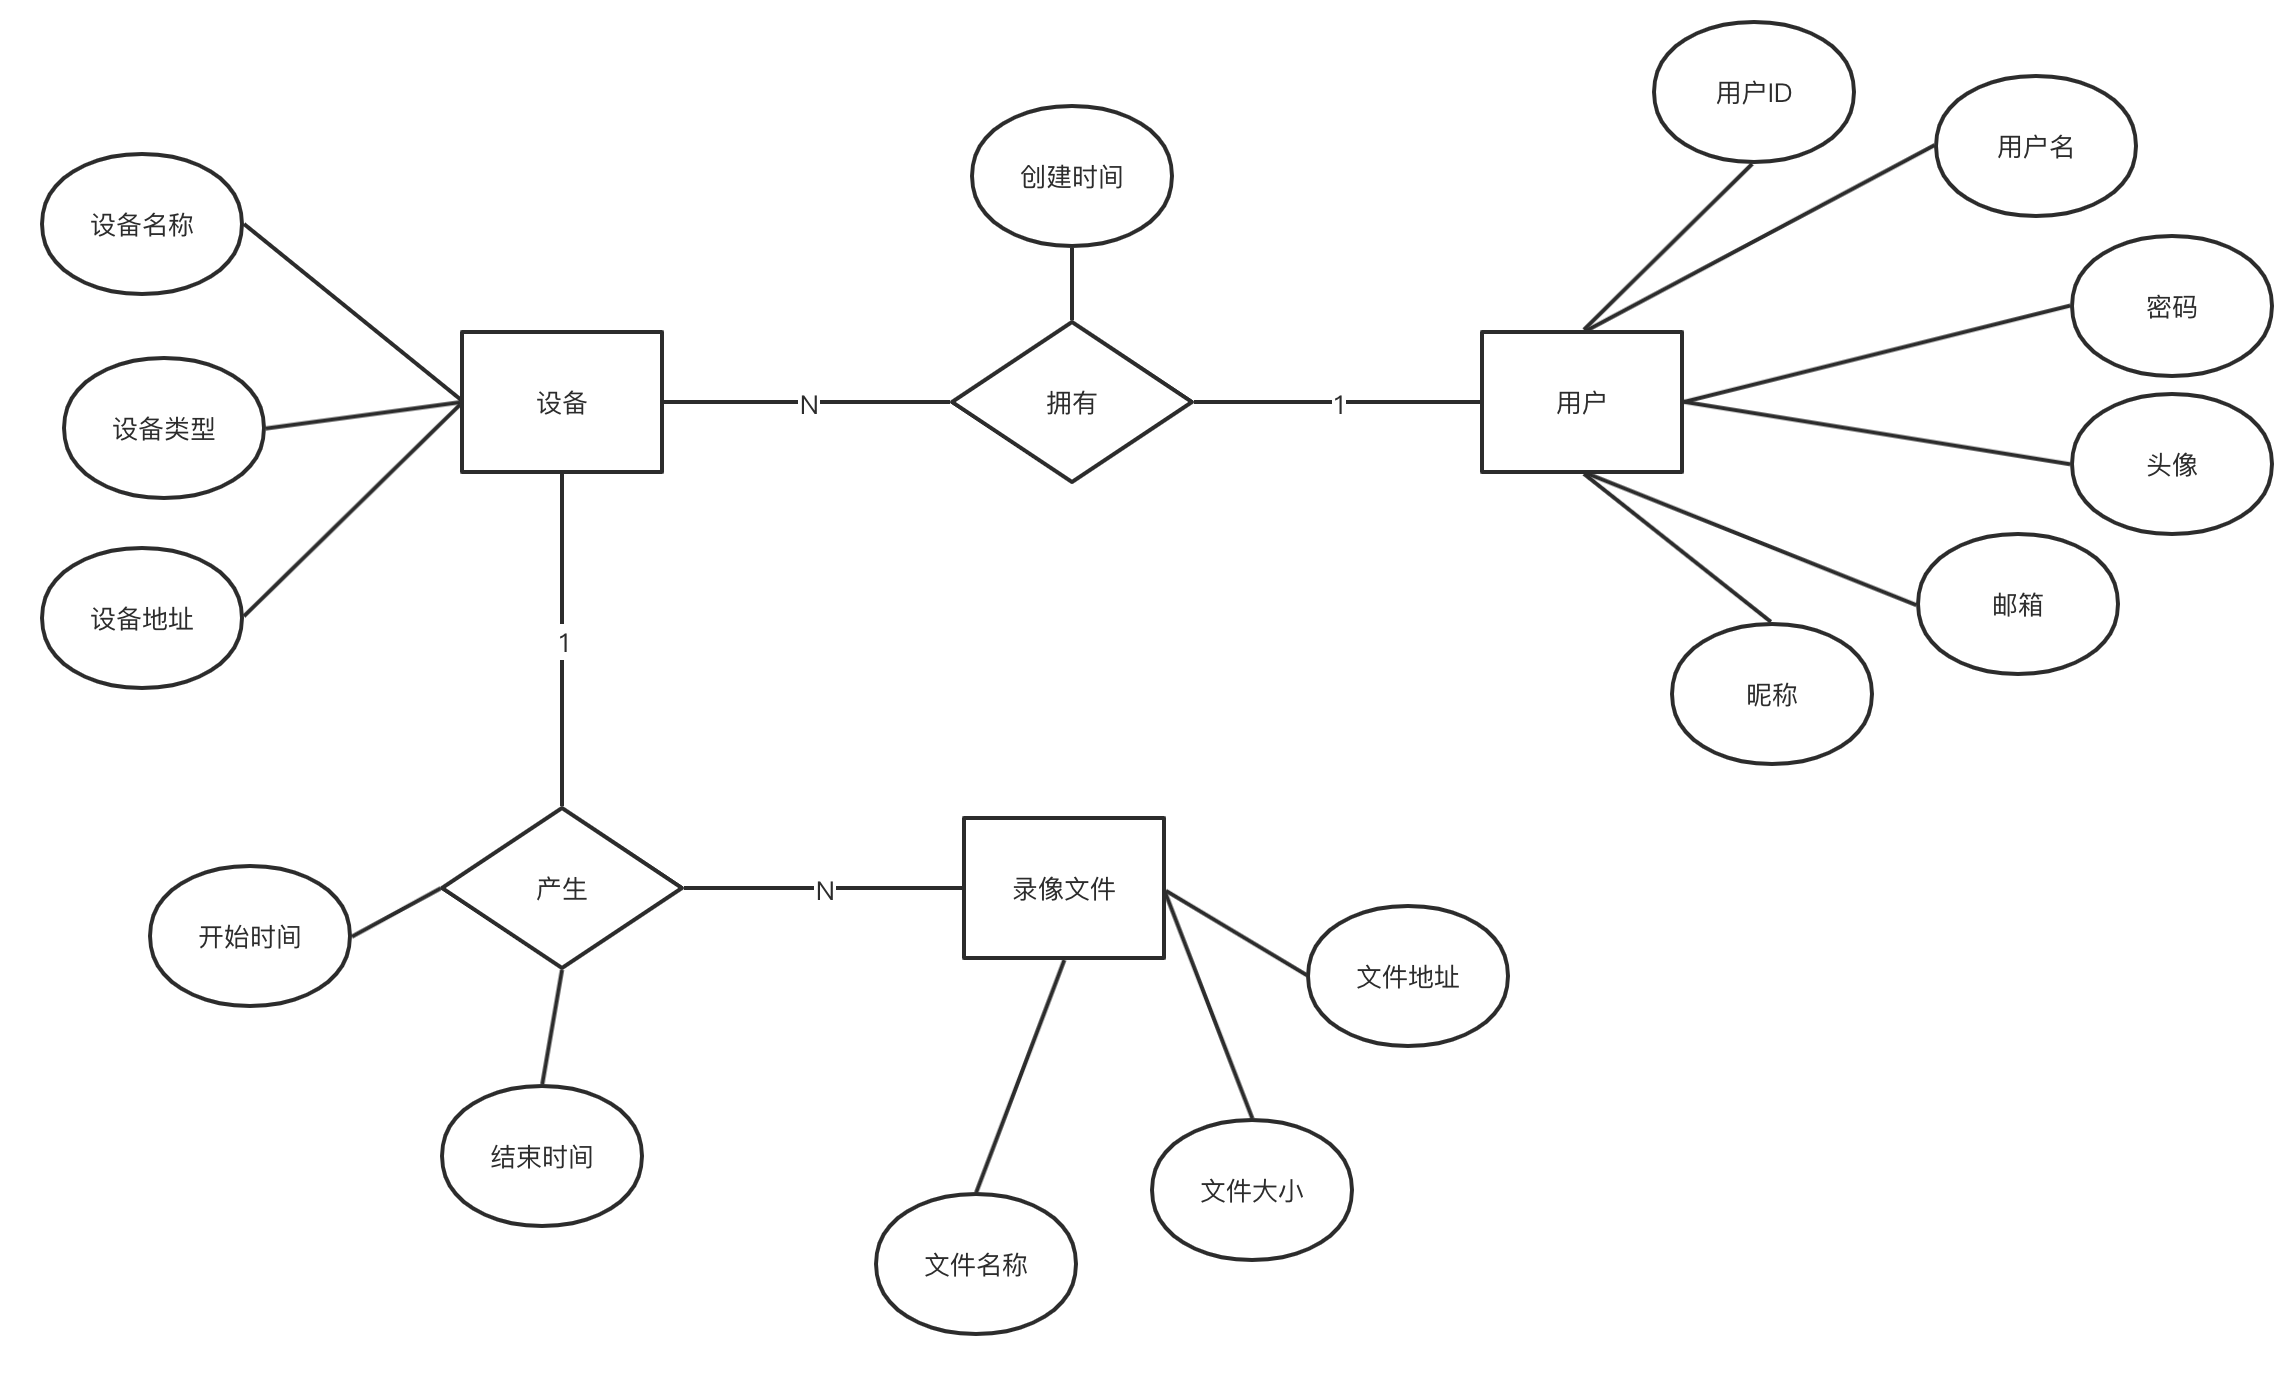
\includegraphics[scale=.3]{./Figure/IMG_erd.png}
    \caption{实体关系图}\label{Fig:erd}
\end{figure}

通过实体关系图,可以推导出数据库表结构和表关系,同样如下图所示。

\begin{figure}[ht]
    \centering
    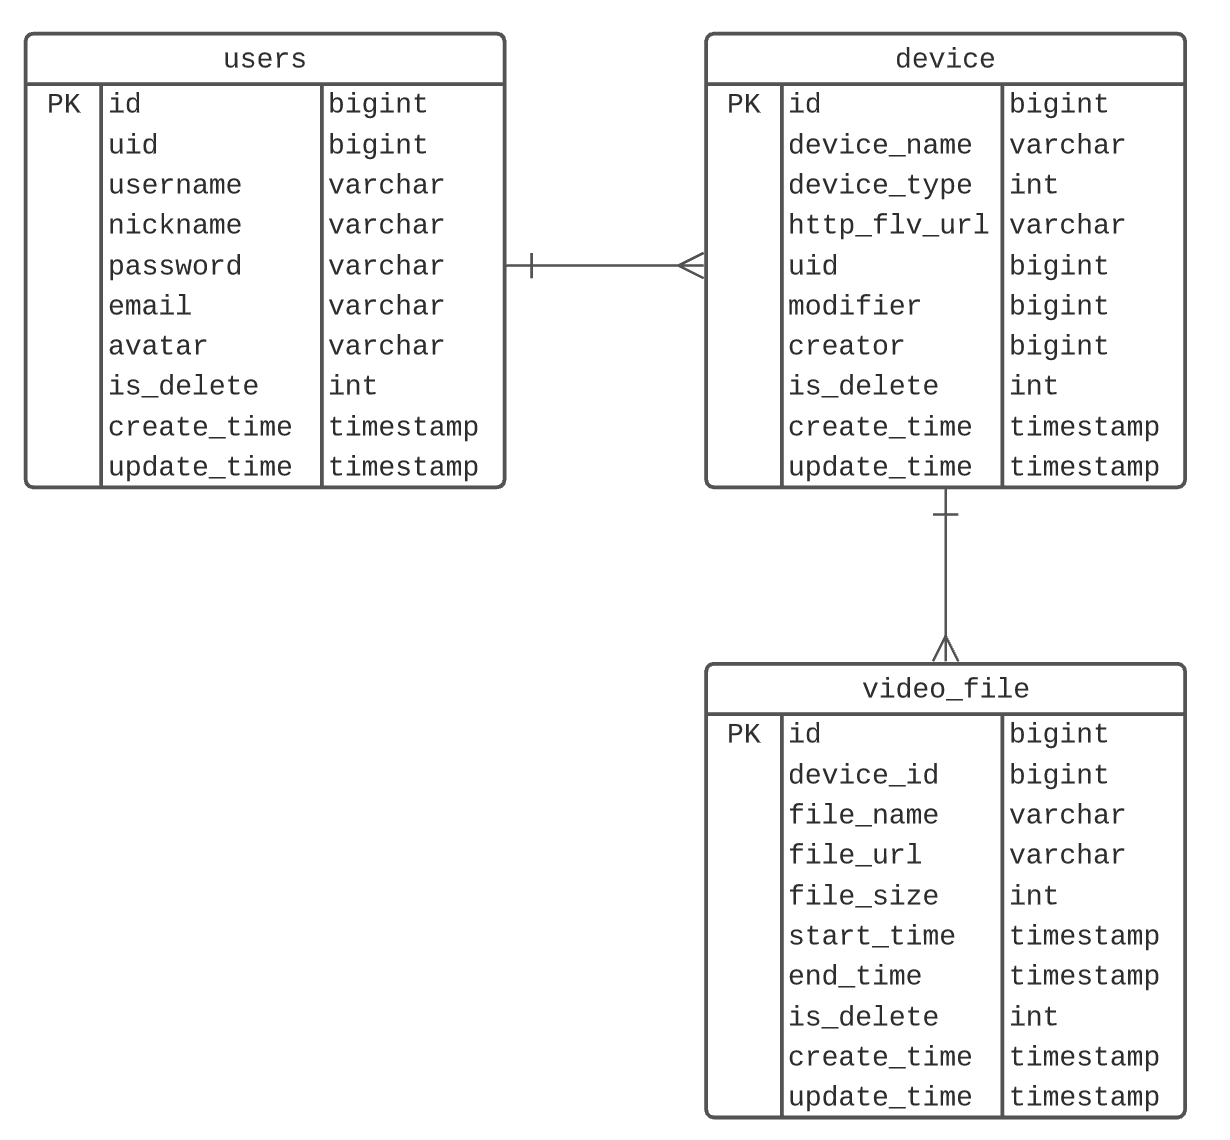
\includegraphics[scale=.6]{./Figure/IMG_db.png}
    \caption{数据库表结构和表关系}\label{Fig:db}
\end{figure}

\section{交互接口设计}

\section{系统模块设计}
系统设计分为五个模块,如下表所示


\begin{longtable}[c]{C{5cm}C{7cm}}
    \caption{这是一个长表格}\label{Tab:longtable}\\
    \hline
    模块名称 & 模块功能\\
    % \hline
    % monitoring-system-common&提供公共工具的能力\\ %公共模块
    % \hline
    % monitoring-system-repo&提供数据存储的能力\\ %数据存储模块
    % \hline
    % monitoring-system-service&系统的主要业务逻辑\\ % 业务逻辑模块
    % \hline
    % monitoring-system-media&离线视频文件的存取\\ % 视频文件存取模块
    % \hline
    % monitoring-system-web&为前端提供接口交互\\ %前端接口交互模块
    % \hline

    \hline
    公共模块&提供公共工具的能力\\ %
    \hline
    数据存储模块&提供持久组件的读写的能力\\ %
    \hline
    业务逻辑模块&系统的主要业务逻辑\\ % 
    \hline
    视频文件存取模块&离线视频文件的存取\\ % 
    \hline
    前端接口交互模块&为前端提供接口交互\\ %
    \hline
\end{longtable}
\subsection{公共模块}
公共模块(monitoring-system-common)提供公共工具的能力。
模块内主要包括开发过程中需要用到的注解(annotation)、常量(constant)、枚举(enumerate)、
异常(exception)以及公共的工具封装(utility)。

公共模块中封装的工具包括时间转换工具类、HTTP请求工具类、Spring工具类以及登陆验证码工具类。

时间转换工具类提供将java.util.Date对象转为具有一定格式的字符串(例如“yyyy-MM-dd HH:mm:ss”),
同时也提供逆向转换的能力,即将字符串格式的时间转化为java.util.Date对象。
% 为什么需要

HTTP请求工具类封装了HTTP请求中相关的GET、POST两种请求方法,借助第三方依赖OkHttp二次开发实现。
支持带参数的GET请求、带请求体参数的POST请求。

Spring工具类提供了对Spring上下文的ApplicationContext的静态访问,
可以在全局状态下任何一个地方访问上下文,即可以访问容器内管理的对象和使用Spring提供的观察者模式。

登陆验证码工具类主要提供在登录时生产验证码图片,如下图所示。

\begin{figure}[ht]
    \centering
    
\includegraphics[width=0.5\linewidth]{./Figure/IMG_code.png}
    \caption{登陆验证码}\label{Fig:code}
\end{figure}

\subsection{数据存储模块}
数据存储模块(monitoring-system-repo)提供持久组件的读写的能力。持久组件就是提供数据存储的服务,
在本系统的设计中,持久组件包括MySQL数据库、Reids内存数据库、本地文件系统。

系统设计使用 Mybatis 框架对数据库进行访问,因此该模块中的大部分代码有时有 Mybatis-Generator
自动生成,包括实体对象类、Mapper接口和Mapper配置文件。除此之外,该模块还包括了各种实体的封装类,
比如前端参数封装类(用于封装前端传递给后端的参数)、HTTP响应类(封装后端接口返回对象)
以及各个模块使用的实体类(VO、BO)。

该模块还负责对象之间的转换,即将VO转换成BO或者将BO转换成BO等。该功能是通过对象拷贝技术MapStruct生成的对象转换代码实现的。

\subsection{业务逻辑模块}
业务逻辑模块(monitoring-system-service)提供业务逻辑处理的功能。
该模块是本系统最核心的一个模块,主要负责业务模块的逻辑应用设计,支持登陆鉴权、设备信息的增删改查、个人信息修改等。

业务逻辑模块的主要设计思路是面向接口编程。
接口主要用于描述类具有什么功能,而并不给出每个功能的具体实现。
一个类可以实现一个或多个接口,并在需要接口的地方,随时使用实现了相应接口的对象。

首先设计接口,再设计其对应的实现的类,接着利用Spring的依赖注入特性,
就可以在上层模块声明接口类型的变量,而无需关心其具体实现。
换句话说,业务逻辑模块的变动不会对上层模块的调用产生任何影响。

这就是软件六大设计原则之一的依赖倒置原则,即面向接口编程。
上层模块不应该依赖底层模块,它们都应该依赖于抽象。
抽象不应该依赖于细节,细节应该依赖于抽象。
上层模块不应依赖底层模块,即上层的业务模块不应该依赖底层的实现模块。
如:人出行使用交通工具,只需要知道是交通工具就可以,不用知道是哪种具体的交通工具。
抽象不应该依赖于细节,细节应该依赖于抽象。
在具体的Java编程中,抽象指代接口、抽象函数,统称为接口,而细节指代接口的具体实现。

\subsection{视频文件存取模块}
视频文件存取模块(monitoring-system-media)提供实时监控视频录制和离线查看检索功能。
该模块提供了两个HTTP的接口,分别是监控回放文件的列表查询接口和监控回放文件下载接口。
对于已经在本系统中绑定的监控摄像头设备,每隔一分钟视频文件存取模块会执行定时任务,
对该设备进行录制,并且录制的时长为80秒,目的是做到前后视频文件能有重合部分,防止视频数据丢失。

对于视频文件的存放,可以在本地文件系统和云存储之间无缝切换。
云存储采用阿里云的OSS对象存储服务或本地搭建的Hadoop分布式存储系统。
对于视频文件的读取,该模块提供了一个GET 方法的HTTP接口,入参为视频文件的名称,返回值为该文件内容。
同时还提供搜索功能,支持按照监控视频的开始时间和结束时间进行范围查找。


\subsection{前端接口交互模块}
前端接口交互模块(monitoring-system-web)提供与前端交互的能力。
该模块负责接受前端的请求,然后调用下层模块(如视频文件存取模块)提供的接口方法,实现业务逻辑,
然后将下层模块的返回值进行一定程度的封装后返回给前端进行展示。





\section{权限系统设计}



























\chapter{系统实现}
